
\item A point moves with deceleration along the circle of radius \( R \) so that at any moment of time its tangential and normal accelerations are equal in moduli. At the initial moment \( t = 0 \) the velocity of the point equals \( v_0 \). Find:
    \begin{center}
        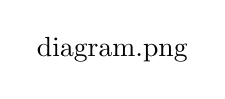
\begin{tikzpicture}
            \node at (0, 0) {diagram.png};
        \end{tikzpicture}
    \end{center}
    \begin{enumerate}
        \item the velocity of the point as a function of time and as a function of the distance covered \( s \);
        \item the total acceleration of the point as a function of velocity and the distance covered.
    \end{enumerate}
